\documentclass{article}

\usepackage{graphicx}
\usepackage{tikz}
\usepackage{tikzsymbols}
\usetikzlibrary{calc,patterns,shapes.geometric}
\pagestyle{empty}
\usepackage[margin=0pt]{geometry}
\geometry{papersize={14in,12in}}

\def\centerarc[#1](#2)(#3:#4:#5){\draw[#1] ($(#2)+({#5*cos(#3)},{#5*sin(#3)})$) arc (#3:#4:#5);}

\begin{document}
	\begin{figure}
		\centering
		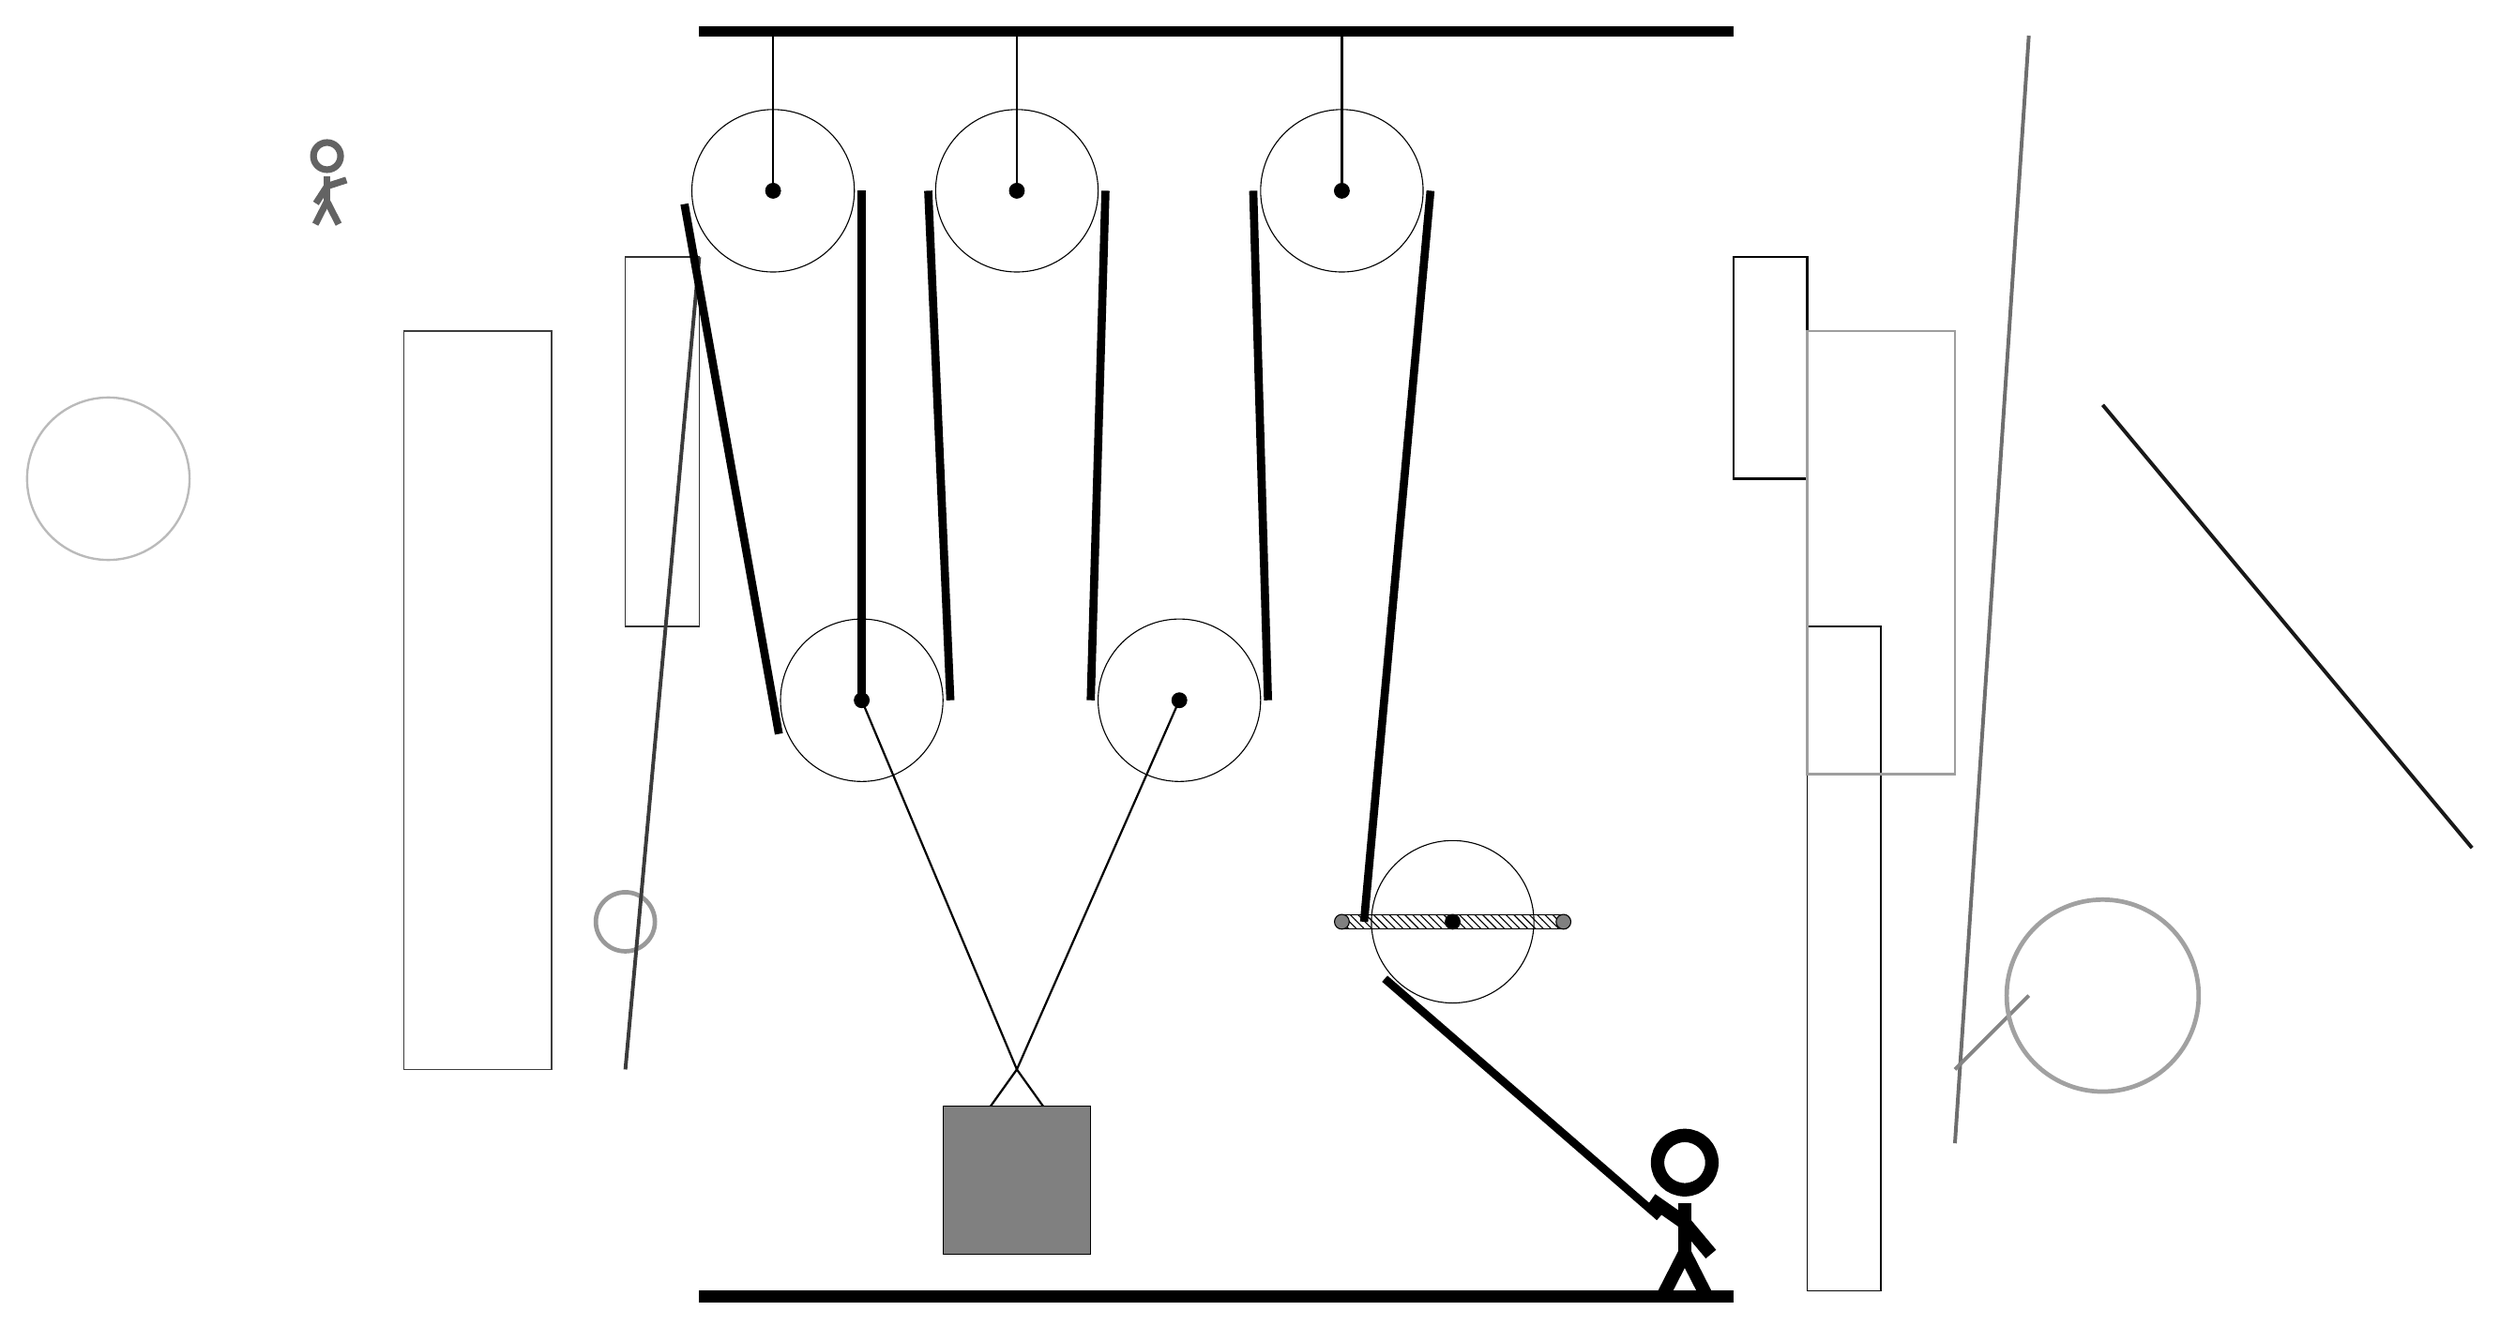
\begin{tikzpicture}
			%%%%% START %%%%%
			
			\draw[fill=black] (-2, 14) rectangle (12, 14.125);
			
			\draw (-1, 11.9) circle (1.1);
			\draw[fill=black] (-1, 11.9) circle (0.1);
			\draw[thick] (-1, 11.9) -- (-1, 14);
			
			\draw[line width=0.5mm, color=black!90](17, 9) -- (22, 3);
			
			\draw[line width=0.5mm, color=black!57](16, 14) -- (15, -1);
			\draw[line width=0.2mm, color=black!80] (-3, 11) rectangle (-2, 6);
			\draw [line width=0.6mm, color=black!40](-3, 2) circle (0.4);
			
			\draw[line width=0.2mm, color=black!97] (14, -3) rectangle (13, 6);
			\draw[line width=0.5mm, color=black!77](-3, 0) -- (-2, 11);
			\draw [line width=0.3mm, color=black!27](-10, 8) circle (1.1);
			\draw[line width=0.2mm, color=black!76] (-4, 0) rectangle (-6, 10);
			\draw[line width=0.3mm, color=black!89] (14, -3) rectangle (14, -3);
			\draw[line width=0.3mm, color=black!98] (13, 11) rectangle (12, 8);
			\draw[line width=0.5mm, color=black!48](16, 1) -- (15, 0);
			
			\draw [line width=0.6mm, color=black!37](17, 1) circle (1.3);
			\draw[line width=0.3mm, color=black!38] (13, 4) rectangle (15, 10);
			
			\node[line width=0.3mm, color=black!61] at (-7, 12) {\Strichmaxerl[5][57][18]};
			
			\draw (2.3, 11.9) circle (1.1);
			\draw[fill=black] (2.3, 11.9) circle (0.1);
			\draw[thick] (2.3, 11.9) -- (2.3, 14);
			
			\draw (6.7, 11.9) circle (1.1);
			\draw[fill=black] (6.7, 11.9) circle (0.1);
			\draw[thick] (6.7, 11.9) -- (6.7, 14);
			
			\draw (0.2, 5) circle (1.1);
			\draw[fill=black] (0.2, 5) circle (0.1);
			
			\draw (4.5, 5) circle (1.1);
			\draw[fill=black] (4.5, 5) circle (0.1);
			
			\draw (8.2, 2) circle (1.1);
			\draw[fill=black] (8.2, 2) circle (0.1);
			\draw[pattern=north west lines, pattern color=black] (6.7, 2.1) rectangle (9.7, 1.9);
			\draw[fill=black!50] (6.7, 2) circle (0.1);
			\draw[fill=black!50] (9.7, 2) circle (0.1);
			
			\draw[thick] (0.2, 5) -- (2.3, 0)  -- (4.5, 5);
			\draw[thick]  (1.8, -0.7) -- (2.3, 0) -- (2.8, -0.7);
			\draw[fill=black!50] (1.3, -0.5) rectangle (3.3, -2.5);
			
			\draw[line width=1.1mm] (0.2, 5) -- (0.2, 11.9);
			\centerarc[line width=1.1mm](-1, 11.9)(0:200:1.2000000000000002);
			\draw[line width=1.1mm] (-2.2, 11.72) -- (-0.922, 4.544);
			\centerarc[line width=1.1mm](0.2, 5)(200:360:1.2000000000000002);
			\draw[line width=1.1mm](1.4, 5) -- (1.1, 11.9);
			\centerarc[line width=1.1mm](2.3, 11.9)(0:180:1.2000000000000002);
			\draw[line width=1.1mm] (3.5, 11.9) -- (3.3, 5);
			\centerarc[line width=1.1mm](4.5, 5)(180:360:1.2000000000000002);
			\draw[line width=1.1mm] (5.7, 5) -- (5.5, 11.9);
			\centerarc[line width=1.1mm](6.7, 11.9)(0:180:1.2000000000000002);
			\draw[line width=1.1mm](7.9, 11.9) --  (7.0, 2);
			\centerarc[line width=1.1mm](8.2, 2)(180:220:1.2000000000000002);
			\draw[line width=1.1mm](7.2808, 1.2286) -- (11, -2);
			
			\node at (11.3, -2) {\Strichmaxerl[10][-35][-50]};
			
			\draw[fill=black] (-2, -3) rectangle (12, -3.15);
			
			%%%%% END %%%%%
		\end{tikzpicture}
	\end{figure}	
\end{document}